\documentclass{beamer}

\usepackage{color}
%\usepackage{beamerthemesplit}
%\usepackage{beamerthemeMalmoe}
%\beamertemplatetransparentcovereddynamic
\mode<presentation>
{
  \setbeamertemplate{background canvas}[vertical shading][bottom=gray!10,top=blue!10]
  \usetheme{Warsaw}
  %\useoutertheme{infolines}
  \usenavigationsymbolstemplate
}

\usepackage{listings}
\usepackage{comment}
\usepackage{amssymb}
\usepackage{amsmath}

\lstset {
  basicstyle=\footnotesize\sffamily,
  tabsize=3
}

\lstdefinelanguage{aadl} {
  morekeywords={in,out,package,end,bus,data,thread,port,group,process,processor,
    system,memory,device,subprogram,public,private,event,property,set,applies,to,
    units,type,implementation,parameter, reference},
  morekeywords={properties,features,annex,modes,connections,flows,
    subcomponents,calls,binding},
  morekeywords={aadlinteger,aadlboolean,aadlstring,aadlfloat},
  morecomment=[l]{--},
}

\newcommand{\MM}[1]{\ensuremath{#1}}

\newcommand{\REGLE}[3]{
%  \box{
    \MM{
      \dfrac{\begin{array}{l} #1 \end{array}}
	    {\begin{array}{l} #2 \end{array}}
    }
%  }
  %\vspace{1mm}
    \begin{left}
      \hbox{#3}
    \end{left}
}
                               
\newcommand{\regle}[2]{
  \MM{
    \frac{\begin{array}{c} #1 \end{array}}
         {\begin{array}{l} #2 \end{array}}
  }
}

\newcommand{\formatreg}[1]{
  \begin{center}
%  \begin{tabular}{|c}
%    \hline
    \vspace{0.5mm}
    \fbox{#1}\\
%    \hline
%  \end{tabular}
  \end{center}
}

\newcommand{\Fait}[1]{\MM{\ \ \xrightarrow{#1}}}

\newcommand{\fait}[1]{\MM{\xrightarrow{\ \ #1}}}

\newcommand{\Faitv}[1]{\MM{\ \xrightarrow{#1}\ }}

\newcommand{\RL}[1]{\,\frac{}{\,^{{#1}}\,}\,}

\newcommand{\RS}[1]{\,\frac{}{^{{#1}}}\,}

\newcommand{\sqplus}{\ {\scriptstyle {\widehat{+}}}\ }

\newcommand{\smplus}{\ {\scriptstyle {\dot{+}}}\ }

\newcommand{\intrupt}{\,{\scriptstyle\leadsto}\,}

\newcommand{\rget}{\frac{}{\text{\ttfamily\ Get\ }}}

\newcommand{\rset}{\frac{}{\text{\ttfamily\ Set\ }}}

\newcommand{\rgvt}{\MM{ \frac{}{\text{\ttfamily\  Await\_Event\ }} }}

\newcommand{\rsvt}{\frac{}{\text{\ttfamily\ Send\_Event\ }}}

%\newcommand{\mget}{\frac{}{{\scriptsize{\text{\ttfamily\ Get\ }}}}

%\newcommand{\mset}{\frac{}{\text{\ttfamily\ Set\ }}}

\newcommand{\mgvt}{\frac{}{\text{\ttfamily\ \ Await\_Event\ }}}

\newcommand{\msvt}{\frac{}{{\text{\ttfamily\ \tiny Send\_Event\ }}}}

\newcommand{\rx}{\frac{}{\large \ x \ }}

\newcommand{\smcirc}{{\scriptscriptstyle \circ}}

\newcommand{\smodot}{{\scriptscriptstyle \odot}}

\newcommand{\smoplus}{\,{\scriptstyle \oplus}\,}

\newcommand{\SFT}[1]{\text{\sffamily #1}}

\newcommand{\FNT}[1]{\text{\footnotesize #1}}

\newcommand{\SC}[1]{$\text{\scshape{#1}}$}

\newcommand{\simu}{Simulink$^{\circledR}$}
\definecolor{LightGray}{rgb}{0.75,0.75,0.75}

\AtBeginSection[]
{
  \begin{frame}<beamer>
    \frametitle{Plan}
    \tableofcontents[current]
  \end{frame}
}

\setcounter{tocdepth}{1}

\title[Automatic Code Gen. \&
  Verif. of HRT Systems.---Page \theframenumber/\inserttotalframenumber]{Automatic Code Generation and
  Verification for Hard Real-time Systems}

\author{Irfan HAMID}

\date{$30^{th}$ May, 2008}

\subtitle{Doctoral dissertation}

\institute[ENST]{\'Ecole Nationale Sup\'erieure des T\'el\'ecommunications}

\begin{document}

\begin{frame}
  \titlepage
\end{frame}

%\frame {
%  \frametitle{Outline}
%  \tableofcontents
%}

\section{Introduction}

\subsection{Context \& background}
\frame {
  \frametitle{Real-time systems}
  \begin{definition}
    A \alert{real-time} system is one in which the validity of a
    computation is dependant not only on the result of said
    computation, but also on the time it is available
  \end{definition}
  \pause
  \begin{center}
    $\includegraphics[scale=0.8]{../figs/hard_vs_soft}$
  \end{center}
}

\frame {
  \frametitle{Code generation}
  \begin{itemize}
    \item When code is not written by hand, it is code generation
    \item Can't come out of thin air
    \pause
    \item Comes from a \alert{model}
  \end{itemize}
  \pause
  \begin{definition}
    A \alert{model} is an abstraction of a system
  \end{definition}
  \textbf{System:} Cannonball fired from a cannon\\
  \textbf{Model:} Equation of projectile with bound variables\\
  \textcolor{gray}{\textbf{Meta-model:} Equation of projectile with
    unbound variables}\\
  \textcolor{LightGray}{\textbf{Meta-meta-model:} Calculus}
}

\frame {
  \frametitle{Software models and MDE (Model Driven Engineering)}
  \begin{itemize}
    \item Software is also approximated by models
    \item Old idea, now evolving into something quite useful
      \pause
    \item Flowcharts$\to$JSD$\to$OMT \& OOSE$\to$UML
    \item Models becoming part of SDLC (S/W Dev. Lifecycle)
    \item Mainly the design and coding part is affected by MDE
    \item To a lesser extent also testing and deployment
    \item Lots of modeling methods, most prevalent example: UML
  \end{itemize}
}

\frame {
  \frametitle{S/W Development Lifecycle: The MDE approach}
  \begin{center}
    $\includegraphics[scale=0.7]{../figs/mde_presentation_generic}$
  \end{center}
}

\frame {
  \frametitle{Verification}
  \begin{itemize}
    \item Use a mathematically precise way to describe a system
    \item Run the mathematical description of the system
    \item Explore \emph{all} possible states the system can go into
    \item Determine whether/which properties hold in which states
    \item Reason based on those properties
  \end{itemize}
}

\frame {
  \frametitle{Context of work}
  But what did \emph{you} do?
  \pause
  \begin{itemize}
    \item Worked in ASSERT European Project
    \item Large consortium, to do what?
      \pause
    \item To use formal methods and MDE to make more robust real-time
      software
  \end{itemize}
  \pause
  OK, but what \emph{part} did you do?
  \pause
  \begin{itemize}
    \item Use a new architecture description language to generate code
      for hard real-time systems
    \item Perform some verifications on the code generated
  \end{itemize}
}

\frame {
  \frametitle{What modeling language? What executive?}
  Code generation from the AADL...
  \pause
  \begin{itemize}
    \item Architecture Analysis \& Design Language (V1, 2004)
    \item Descendant of MetaH
    \item Tailored to the real-time and safety-critical domain
    \item Developed by SAE
  \end{itemize}
  \pause
  ... to the Ada Ravenscar Profile
  \begin{itemize}
    \item Ada Ravenscar, a profile (subset) of Ada
    \item Intended for use in high-integrity hard real-time systems
    \item Provides certain safety guarantees and analysis possibilities
  \end{itemize}
}

\frame {
  \frametitle{A picture is worth...}
  $\includegraphics[scale=0.7]{../figs/mde_presentation}$
}

\subsection{Survey}

\frame {
  \frametitle{Aren't there others?}
  Of course there are, I even showed some
  \pause
  \begin{itemize}
    \item Dozens of modeling methodologies
    \item Some mainstream, some niche
    \item Some famous, some unknown
      \pause
    \item Ones pertinent to the domain
      \begin{itemize}
        \item UML
        \item UML profiles
        \item SCADE, Simulink
      \end{itemize}
  \end{itemize}
}

\frame {
  \frametitle{UML}
  \begin{itemize}
    \item General purpose modeling language
    \item Initially a graphical representation for OO concepts
    \item Now has concepts like functional modeling \& decomposition
    \item Tools like Rhapsody furnish a modicum of RT support
  \end{itemize}
  \pause
  \textbf{Advantages}
  \begin{itemize}
    \item Inclusionist approach, accomodates everyone, allows
      extensions (which is why it's a good PIM)
    \item Some support for real-time from Rhapsody and similar tools
  \end{itemize}
  \pause
  \textbf{Disadvantages}
  \begin{itemize}
    \item Complex compared to AADL, ambiguous semantics
    \item Strongly tied to OO concepts
    \item Absence of runtime constructs, needs \alert{semantic
      overloading}
  \end{itemize}
}

\frame {
  \frametitle{HRT-UML}
  \begin{itemize}
    \item{A profile of UML for hard real-time systems}
    \item{Closely tied to the Ravenscar Profile for HI systems}
    \item{\emph{Stereotypes} like {\footnotesize $\ll PERIODIC\gg$, $\ll
        SPORADIC\gg$}}
    \item{{\footnotesize PERIOD, DEADLINE, PRIORITY} become meta-attributes}
  \end{itemize}
  \pause
  \textbf{Advantages}
  \begin{itemize}
    \item Explicit modeling of HRT concepts
    \item Ravenscar Profile$\implies$safety
    \item Allows \emph{a priori} schedulability analysis
  \end{itemize}
  \pause
  \textbf{Disadvantages}
  \begin{itemize}
    \item Enforces a low level of abstraction
    \item Engages in more \alert{semantic overload}
  \end{itemize}
}

\frame {
  \frametitle{Lustre \& SCADE Suite}
  \begin{itemize}
    \item{Synchronous data flow programming language}
    \item{Primary use in reactive and control systems}
    \item{System is set of \alert{nodes}, operate in lockstep}
    \item{SCADE Suite, an industrial version of the language}
  \end{itemize}
  \pause
  \textbf{Advantages}
  \begin{itemize}
    \item Mathematically sound, allows model checking
    \item Good abstraction level of control system concepts
    \item Robust, deterministic execution
  \end{itemize}
  \pause
  \textbf{Disadvantages}
  \begin{itemize}
    \item Synchronous execution model, cyclic executive
    \item No aperiodic threads, all periods harmonic
    \item Not suited to general real-time systems
  \end{itemize}
}

%%%%%%%%%%%%%%%%%%%%%%%%%%%%%%%%%%%%%%%%%%%%%%%%%%%%%
\begin{comment}

\frame {
  \frametitle{Lustre \& SCADE Suite}
  %\begin{minipage}{0.45\linewidth}
    \textbf{Advantages}
    \begin{itemize}
      \item{Mathematically sound method}
      \item{Provides robust \& deterministic execution}
      \item{Provides direct abstraction of control system concepts at
        software level}
      \item{Model checking possible because of internal automata-based
        representation}
    \end{itemize}
  %\end{minipage}
  %\hspace{2mm}
  %\begin{minipage}{0.45\linewidth}
    \pause
    \textbf{Disadvantages}
    \begin{itemize}
      \item{Is a synchronous, thus implemented via a cyclic executive,
        which precludes true aperiodic tasks}
      \item{Potential wastage of processor cycles}
      \item{Implies zero execution time semantics}
      \item{Not well-suited to real-time systems other than control
        systems}
    \end{itemize}
  %\end{minipage}
}

\frame {
  \frametitle{HRT-UML (contd.)}
  %\begin{minipage}{0.45\linewidth}
    \textbf{Advantages}
    \begin{itemize}
      \item{Folds the design into UML}
      \item{Explicit modeling of hard real-time constructs}
      \item{\emph{Might} allow inclusion of functional modeling via
        statecharts}
      \item{Offline, \emph{a priori} schedulability analysis}
    \end{itemize}
  %\end{minipage}
  \hspace{2mm}
  %\begin{minipage}{0.45\linewidth}
    \pause
    \textbf{Disadvantages}
    \begin{itemize}
      \item{Folds the design into UML}
      \item{More semantic overload than vanilla UML}
      \item{Enforces a low level of abstraction for concepts. Is a
        graphical representation of the software concepts}
    \end{itemize}
  %\end{minipage}
}

\frame {
  \frametitle{Requirements}
  \begin{minipage}{0.45\linewidth}
    \begin{itemize}
      \item<1->{\alert{Functional}}
      \item<2->{\alert{Non-functional}}
    \end{itemize}
  \end{minipage}
  \hspace{2mm}
  \begin{minipage}{0.45\linewidth}
    \begin{itemize}
      \item<1->{$y = f(x)$}
      \item<2->{Timing, memory, GUI$\ldots$}
    \end{itemize}
  \end{minipage}
  \vspace{3mm}
  \pause
  \pause
  \begin{itemize}
    \item{Traditional systems place premium on functional
      requirements}
    \item{Breach of functional requirements breaks \emph{mission}}
    \item{A word processor that does not save a file}
      \pause
      \vspace{3mm}
    \item{Breach of non-functional requirements \emph{may} be
      inconvenience}
    \item{\emph{May} be more than a mere inconvenience}
    \item{A word processor that saves a file in 30 secs}
  \end{itemize}

  \pause
  \begin{definition}
    The \alert{validity} of a computational result is the inverse of
    the amount of deviation it causes from the system's set of
    requirements
  \end{definition}
}

\subsection{Real-time systems}
\begin{frame}
  \frametitle{Real-time systems}
  \begin{minipage}{0.4\linewidth}
    \begin{itemize}
      \item<1->{Traditional}
      \item<2->{Real-time}
    \end{itemize}
  \end{minipage}
  \begin{minipage}{0.56\linewidth}
    \begin{itemize}
      \item<1->{$Result\ validity = f (value)$}
      \item<2->{$Result\ validity = f (value, time)$}
    \end{itemize}
  \end{minipage}
  \vspace{3mm}
  \pause
  \pause
  \begin{definition}
    A \alert{real-time} system is one in which the validity of a
    computation is dependant not only on the result of said
    computation, but also on the time it is available
  \end{definition}

  \pause
  \begin{itemize}
    \item{Industrial process control \& monitoring}
    \item{Vehicular and platform control}
    \item{Vehicular status monitoring and sensors (GPS etc.)}
    \item{Multimedia systems}
  \end{itemize}
\end{frame}

\frame {
  \frametitle{Classes of real-time systems}
  \begin{center}
    \uncover<1->{$\includegraphics[scale=0.8]{../figs/hard_vs_soft}$}
    \uncover<2->{$\includegraphics[scale=0.6]{../figs/rt_apps_overview}$}
  \end{center}
}

\subsection{High-integrity \& safety-critical software}
\frame {
  \frametitle{HI and SC software}
  \begin{description}
    \item[High-integrity:]{Software on which are leveraged stringent
      requirements of correctness, robustness \& availability}
    \item[Safety-critical:]{Software on which a fault \alert{may}
      endanger human life}
  \end{description}
  \begin{itemize}
    \item<2->{Vehicular management (cruise control, autopilot)}
    \item<2->{Assembly lines}
    \item<3->{Medical devices (radiation machines, X-rays, MRIs)}
    \item<3->{Mission management systems (GNC, GPS, $\ldots$)}
    \item<4->{Control systems (fly-by-wire, drive-by-wire, anti-lock
      braking)}
  \end{itemize}
  \pause
  \begin{block}{Why?}
    \begin{itemize}
      \item<2->{Reduction of labor via automation}
      \item<3->{Introduction of functionality}
      \item<4->{Maintaining platform stability}
    \end{itemize}
  \end{block}
}

\frame {
  \frametitle{Certification}
  \begin{itemize}
    \item{Most safety-critical software is \alert{certified}}
    \item{Certification entails an audit by a---usually
      government---agency}
    \item{Certification is necessary for deployment of software}
    \item{Certification may be achieved via
      \begin{itemize}
        \item{Manual inspection of code}
        \item{Formal verification}
        \item{Proofs}
      \end{itemize}
    }
      \pause
    \item{ANS7432: Application Criteria for Safety Systems of Nuclear
      Power Generating Stations}
    \item{DO-178B: Software Considerations in Airborne Systems and
      Equipment Certification}
  \end{itemize}
}

\frame{
  \frametitle{DO-178B \& the SDLC}
  \begin{itemize}
    \item{DO-178B is the certification standard for aerospace
      software}
    \item{Is \alert{not} an SDLC}
    \item{Leverages requirements on each phase of the SDLC chosen}
    \item{Most requirements are documentation, some testing
      requirements as well}
  \end{itemize}
  \pause
  {\footnotesize
  \begin{table}
    \centering
    \begin{tabular}{|l|l|l|}
      \hline
      \textbf{Software level}&\textbf{Failure condition}&\textbf{Outcome}\\
      \hline
      Level A & Catastrophic & Death or injury\\
      Level B & Hazardous/Severe-major & Injury\\
      Level C & Major & Unsafe workload\\
      Level D & Minor & Increased workload\\
      Level E & No effect & None\\
      \hline
    \end{tabular}
    \caption{DO-178B Safety Criticality Levels}
  \end{table}
  }
}

\subsection{Model driven engineering}

\frame {
  \frametitle{Make models, not code}
  Model driven engineering is an approach to development where
  \begin{quote}
    models are the primary artifacts of development and developers
    rely on computer-based technologies to transform models to running
    systems
  \end{quote}
  \pause
  \begin{itemize}
    \item{A model is an approximation or an abstraction of a system}
    \item{It abstracts away complexity, thus is easier to construct}
      \pause
    \item{Models can be used for one of three purposes
      \pause
      \begin{enumerate}
        \item{Documentation}
          \pause
        \item{Analysis}
          \pause
        \item{Code generation}
      \end{enumerate}
    }
  \end{itemize}
}

\frame {
  \frametitle{MDE in SDLC}
  \begin{itemize}
    \item{System requirements are captured}
    \item{Functional specifications are given}
    \item{\alert{System design is constructed}}
    \item{\alert{Code is written---or generated---corresponding to
        design}}
    \item{Modules are tested}
    \item{Modules are integrated}
    \item{System is deployed}
  \end{itemize}
}
\frame {
  \frametitle{MDE in the SDLC}
  \begin{center}
    $\includegraphics[scale=0.78]{../figs/mde_chain}$
  \end{center}
}

\subsection{Motivation and context of contribution}

\frame {
  \frametitle{Handling real-time system complexity}
  \begin{itemize}
    \item{Complexity of real-time systems increasing
      \begin{itemize}
        \item{More complex systems being constructed}
        \item{More functionality being demanded, the \emph{``give me
            more''} effect}
        \item{Vicious circle (more compute power$\to$more
          functionality$\to$more compute power)}
        \item{Faster times-to-market}
      \end{itemize}
    }
    \item{Becoming unfeasible to write code by hand}
    \item{Manual coding increases chances of errors}
    \item{Thus MDE approach even more pertinent for HI, RT systems}
  \end{itemize}
}

\frame {
  \frametitle{Motivation for work}
  \begin{itemize}
    \item{Various MDE approaches exist, some general, some tailored
      for real-time systems}
    \item{\textbf{UML:} general purpose. Tool-dependant support for
      real-time systems, generates functional and framework code}
    \item{\textbf{ADLs:} Architecture Description Languages such as
      Rapide, Write, etc. which provide a higher-level view of
      systems}
      \item{\textbf{UML Profiles:} specializations of UML such as
        MARTE and HRT-UML specifically tailored for real-time systems}
      \item{\textbf{Synchronous:} model-driven synchronous approaches
        such as Lustre and MATLAB \simu that generate control system
        code from high-level system models}
  \end{itemize}
}
\end{comment}

%\section{Survey}
\subsection{Real-time tasks \& schedulers}
\begin{frame}
  \frametitle{Real-time tasks}
  \begin{definition}
    Real-time tasks are the independant or co-dependant units of
    execution that may handle different aspects or axes of the entire
    computational responsibility imposed upon the system under
    separate temporal constraints
  \end{definition}
  \pause 
  \begin{itemize}
    \item{Real-time tasks are almost always recurrent, in that they
      occur iteratively over the lifetime of the system and one
      \emph{instance} of a task is called a \emph{job}}
    \item{Tasks are, in effect, containers for jobs or functionality}
  \end{itemize}
\end{frame}

\frame {
  \frametitle{Temporal characteristics of tasks}
  \begin{itemize}
    \item{\textbf{Dispatch protocol:} Time triggered or event
      triggered}
    \item{\textbf{Period (T):} The frequency of time triggered tasks}
    \item{\textbf{Deadline (D):} The instance of time between dispatch
      and completion of a job in nominal functioning of the system}
    \item{\textbf{WCET (C):} Worst Case Execution Time for \emph{any}
      job of a task}
  \end{itemize}
  \pause
  \begin{definition}
    Task \alert{dispatch} is when it is taken from the set of blocked
    tasks and added to the set of ready tasks
  \end{definition}

  \begin{definition}
    Task \alert{release} is when the task is taken from the ready
    queue and put on the processor itself, and thus starts execution
  \end{definition}
}

\frame {
  \frametitle{Time-triggered or periodic tasks}
  \begin{itemize}
    \item{Those that are dispatched as a function of system time}
    \item{Temporal characteristic of \alert{period}}
    \item{Are mostly hard real-time tasks}
    \item{Major uses include
      \begin{enumerate}
        \item{In control systems, periodic tasks carry out the
          computation of the \alert{transfer function}}
        \item{In both control and information/monitoring systems, they
          are used to periodically read sensors}
        \item{Status display updates to provide important information
          to operators}
      \end{enumerate}
    }
  \end{itemize}
}

\frame {
  \frametitle{Event-triggered or aperiodic tasks}
  \begin{itemize}
    \item{Aperiodic tasks are those that are dispatched as a result of
      an event from the environment or another task}
    \item{Aperiodic tasks may overload a system in case of an
      \alert{event storm}}
    \item{Safer version is sporadic task
      \begin{itemize}
        \item{Launched as a function of event arrival \emph{and}
          system time}
        \item{Temporal characteristic of minimum inter-arrival time
          between successive task dispatches}
        \item{Results in a system that is resilient to overload}
      \end{itemize}
    }
    \item{Thus, for safety-critical systems, sporadic tasks are a much
      more attractive option}
  \end{itemize}
}

\frame {
  \frametitle{Real-time schedulers}
  \begin{itemize}
    \item{Scheduler is responsible for task dispatch and release}
    \item{Real-time schedulers make decisions based on temporal
      characteristics of the task set}
    \item{Various real-time schedulers exist
      \begin{itemize}
        \item{Cyclic schedulers}
        \item{Fixed priority preemptive scheduler}
        \item{Earliest deadline first scheduler}
        \item{$\ldots$}
      \end{itemize}
    }
  \end{itemize}
}

\frame {
  \frametitle{Cyclic executives}
  \begin{itemize}
    \item{Oldest real-time scheduling method available}
    \item{Single timer callback calls different functions of the
      system}
    \item{Implies a synchronous system
      \begin{itemize}
        \item{Zero execution time semantics}
        \item{All tasks must be periodic}
        \item{All periods must be harmonic with the \alert{base rate}}
        \item{Assumption that the program reacts to external event
          before other event occurs}
        \item{No preemption, no concurrency control, no race
          conditions}
        \item{Completely deterministic execution}
      \end{itemize}
    }
  \end{itemize}
}

\frame[containsverbatim] {
  \frametitle{Cyclic executives (contd.)}
    \begin{minipage}{0.45\linewidth}
\begin{lstlisting}[language=c]
{
  static int job = 0;
  job++;
  A();
  if(job==2 || job==4) {
    B();
    C();
  }
  if(job==4) {
    D();
    job = 0;
  }
}
\end{lstlisting}
    \end{minipage}
    \hspace{2mm}
    \begin{minipage}{0.45\linewidth}
      $\includegraphics[scale=0.6]{../figs/cyclic_exec}$
    \end{minipage}
}

\frame {
  \frametitle{Process based executives}
  \begin{itemize}
    \item{The ``operating system'' approach}
    \item{Separate processes, each with potentially multiple threads}
    \item{Can be preemptive or non-preemptive}
    \item{Context switching to change tasks on the processor}
    \item{True multi-processing capability}
    \item{Implies a number of things
      \begin{itemize}
        \item{Allows periodic \emph{and} aperiodic tasks}
        \item{Is not restricted to zero execution time semantics}
        \item{Concurrency is possible, thus mutual exclusion required}
        \item{Non-determinism is possible in execution}
      \end{itemize}
    }
    \item{The scheduler decides which task will execute}
  \end{itemize}
}

\frame {
  \frametitle{Fixed Priority Preemptive Scheduling}
  \begin{itemize}
    \item{A simple, robust real-time scheduler}
    \item{The scheduler is launched periodically, and it selects the
      highest priority task among all those that are ready to execute}
    \item{At any time, a lower priority task may be interrupted by a
      higher priority task}
    \item{Task priorities do not change during the lifetime of the
      system}
  \end{itemize}
}

\frame {
  \frametitle{Priority assignments with RMA, RTA}
  \begin{itemize}
    \item{Seminal paper of Leyland \& Liu gives optimum priority
      assignment}
    \item{Rate Monotonic Assignment implies priority assignment in
      inverse order of periods, i.e., fastest task is assigned highest
      priority}
    \item{Basic RMA is for independant tasks, those that do not
      communicate}
    \item{Task interaction can be analyzed by introducing terms in the
      equations (dependant on type of synchronization protocol)}
    \item{More precise (and optimistic) analysis technique or Response
      Time Analysis exists as well}
  \end{itemize}
}

\subsection{Model-driven approaches}

\frame {
  \frametitle{UML}
  \begin{itemize}
    \item{Software design language standardized by the OMG}
    \item{An amalgamation of various methods, OMT, OOSE, Booch}
    \item{It is a large, complex language (13 different diagrams)}
    \item{More or less an elevation of OOP concepts to design level}
    \item{Allows modeling of \alert{classes} and \alert{objects}}
    \item{Important diagrams from the point-of-view of RT systems are
      the class diagram, the statechart and the composite structure
      diagram
      \begin{itemize}
        \item{Class diagrams allow the graphical description of the
          class hierarchy and relation topology among classes}
        \item{Statecharts allow the description of functional behavior
          of classes}
        \item{Composite structure diagrams allow the description of
          hierarchies of composition}
      \end{itemize}
    }
  \end{itemize}
}

\frame {
  \frametitle{UML (contd.)}
  $\includegraphics[scale=0.6]{../figs/class_diag}$
}

\frame {
  \frametitle{UML (contd.)}
  %\begin{minipage}{0.45\linewidth}
    \textbf{Advantages}
    \begin{itemize}
      \item{Standardized, prevalent}
      \item{Close to the software domain}
      \item{Intuitive modeling of OO}
      \item{Intuitive code generation, specially for OO target
        languages}
      \item{Contains extension mechanisms}
    \end{itemize}
  %\end{minipage}
  %\hspace{2mm}
  \pause
  %\begin{minipage}{0.45\linewidth}
    \textbf{Disadvantages}
    \begin{itemize}
      \item{Semantic variation among implementations}
      \item{Very complex}
      \item{Strongly tied to OO concepts!}
      \item{Engages in \alert{semantic overload}}
      \item{No support for hard real-time concepts}
    \end{itemize}
  %\end{minipage}
}

\frame {
  \frametitle{HRT-UML}
  \begin{itemize}
    \item{A profile of UML for hard real-time systems}
    \item{Closely tied to the Ravenscar Profile for HI systems}
    \item{Uses \emph{stereotypes} on classes to represent entities
      like tasks, mutexes, etc.
      \begin{itemize}
        \item{{\tiny $\ll PERIODIC\gg$, $\ll SPORADIC\gg$, $\ll
            PASSIVE\gg$} are tags on classes}
        \item{{\tiny PERIOD, DEADLINE, PRIORITY} etc. become
          meta-attributes of these classes}
      \end{itemize}
    }
    \item{Puts a premium on safety, as it directly models the
      Ravenscar Profile}
    \item{Allows \emph{a priori} feasibility analysis of the system}
  \end{itemize}
}

\frame {
  \frametitle{HRT-UML (contd.)}
  %\begin{minipage}{0.45\linewidth}
    \textbf{Advantages}
    \begin{itemize}
      \item{Folds the design into UML}
      \item{Explicit modeling of hard real-time constructs}
      \item{\emph{Might} allow inclusion of functional modeling via
        statecharts}
      \item{Offline, \emph{a priori} schedulability analysis}
    \end{itemize}
  %\end{minipage}
  \hspace{2mm}
  %\begin{minipage}{0.45\linewidth}
    \pause
    \textbf{Disadvantages}
    \begin{itemize}
      \item{Folds the design into UML}
      \item{More semantic overload than vanilla UML}
      \item{Enforces a low level of abstraction for concepts. Is a
        graphical representation of the software concepts}
    \end{itemize}
  %\end{minipage}
}

\frame {
  \frametitle{Lustre \& SCADE Suite}
  \begin{itemize}
    \item{Lustre is a synchronous data flow programming language}
    \item{Primary use in reactive and control systems}
    \item{System is a set of \alert{nodes} that operate in synchronous
      lockstep}
    \item{SCADE Suite is an industrial version of the language, with
      graphical editing capability}
  \end{itemize}
}

\frame {
  \frametitle{Lustre \& SCADE Suite}
  %\begin{minipage}{0.45\linewidth}
    \textbf{Advantages}
    \begin{itemize}
      \item{Mathematically sound method}
      \item{Provides robust \& deterministic execution}
      \item{Provides direct abstraction of control system concepts at
        software level}
      \item{Model checking possible because of internal automata-based
        representation}
    \end{itemize}
  %\end{minipage}
  %\hspace{2mm}
  %\begin{minipage}{0.45\linewidth}
    \pause
    \textbf{Disadvantages}
    \begin{itemize}
      \item{Is a synchronous, thus implemented via a cyclic executive,
        which precludes true aperiodic tasks}
      \item{Potential wastage of processor cycles}
      \item{Implies zero execution time semantics}
      \item{Not well-suited to real-time systems other than control
        systems}
    \end{itemize}
  %\end{minipage}
}

\section{Building blocks}

%\frame {
%  \frametitle{Technological bricks and mortar}
%  \begin{itemize}
%    \item Code generation entails a tuple $<Source, Target>$
%    \item Source is the Architecture Analysis \& Design Language
%    \item Target language is Ada Ravenscar Profile
%    \item Runtime is the Open Ravenscar Kernel (ORK)
%    \item AADL \& Ravenscar Profile are key technologies
%  \end{itemize}
%}

\subsection[AADL]{Architecture Analysis \& Design Language}
\frame {
  \frametitle{AADL---The background}
  \begin{itemize}
    \item An ADL descendant of MetaH from Honeywell
    \item Major industrial entities are involved
    \item Allows modeling of runtime entities
      \pause
    \item Via components with well-defined interfaces
      \pause
    \item Which are connected together, giving communication toplogy
      \pause
    \item Different \emph{categories} of components
      {\footnotesize
        \begin{tabular}{|l|l|l|}
          \hline
          \textbf{Software} & \textbf{Hardware} & \textbf{Hybrid}\\
          \hline
          Process & Processor & System\\
          Thread & Device & \\
          Thread group & Bus & \\
          Data & Memory & \\
          Subprogram & & \\
          \hline
        \end{tabular}
      }
      \pause
    \item Separation of component interfaces \& implementations
  \end{itemize}
}

\frame {
  \frametitle{AADL---So what can I do with it?}
  \begin{itemize}
    \item Arch. description of apps, using constructs like processes,
      threads, processors etc.
    \item Only \alert{non-functional} aspects can be described
    \item Functional aspects (behavior) defined separately
  \end{itemize}
  \pause
  \begin{center}
    $\includegraphics[scale=0.5]{../figs/comp_code}$
  \end{center}
}

\frame {
  \frametitle{AADL---Component features and properties}
  \begin{itemize}
    \item \alert{Feature} is an interface point on a component
    \item Ports, subprograms, data accesses, subprogram accesses and
      parameters
    \item Features are connected together
      \pause
    \item \alert{Properties} are $<Name, Value>$ pairs attached to
      components
    \item Describe aspects not otherwise expressible
    \item Attached to types, implementations and instances
    \item E.g., \texttt{Dispatch\_Protocol}, \texttt{Period} for
      threads
  \end{itemize}
}

\subsection{Ada Ravenscar Profile}

\frame {
  \frametitle{Ravenscar---High-integrity Profile for Ada}
  \begin{itemize}
    \item The Ada language is rich in tasking constructs
    \item Tasks, and protected objects to let them interact
    \item Rendezvous among tasks also possible
    \item Ravenscar Profile is a restriction of these rich facilities
    \item Restrictions allow \emph{a priori} feasibility analysis
    \item Allow safety property guarantees
      \begin{itemize}
        \item No deadlock
        \item Bounded priority inversion
      \end{itemize}
      \pause
    \item Good choice for hard real-time systems
    \item Sporadic tasks allows protection from \alert{event storms}
  \end{itemize}
}

\begin{comment}
\frame {
  \frametitle{Ravenscar---The Restrictions}
  \begin{itemize}
    \item No creation/destruction of tasks/protected objects
    \item No synchronous communication
    \item All communication/synchronization via protected objects
    \item All protected objects must obey priority ceiling
      protocol
    \item At most one entry per protected object
    \item Data exchange via protected objects with only procedures
    \item Event signaling via protected objects with an entry
    \item \texttt{FIFO\_Within\_Priorities} scheduler, a kind of FFPS
  \end{itemize}
}
\end{comment}

\frame[containsverbatim] {
  \frametitle{Ravenscar---Patterns}
  \emph{Profile not set of patterns, but they are useful guidelines}
       {\footnotesize
         \begin{center}
           \begin{lstlisting}[language=ada,size=\tiny]
task Sporadic is
  Min_Separation : Time_Span;
  Next_Dispatch : Time;
begin
  Min_Separation := Min_Separation_P;
  loop
    Event_Object.Await;
    Next_Dispatch := Clock + Min_Separation;
    -- ... Non-suspending sporadic response code ...
    delay until Next_Dispatch;
  end loop;
end Sporadic;
           \end{lstlisting}
         \end{center}
       }
}


\section{Model to Code Transformations}

\subsection{Rationale}

\frame {
  \frametitle{Rationale---Why generate it automatically?}
  \begin{itemize}
    \item Ada Ravenscar, more tedious than meets the eye
    \item Code generation will reduce this effort
    \item Will result in no (or fewer) errors in the code generated
    \item AADL and Ada Ravenscar, a good \emph{fit}
      \begin{itemize}
        \item Domain specifity of AADL
        \item Intuitive meshing AADL/Ravenscar, similar ``concept
          space''
        \item Industrial acceptance
        \item Reasonable level of abstraction \pause \emph{Yes, I
          explain}
      \end{itemize}
  \end{itemize}
}

\frame {
  \frametitle{Generation of an execution framework}
  \begin{itemize}
    \item AADL system constructs$\implies$``execution
      framework''
    \item \textcolor{gray}{Something like Statecharts
      (functional)$\implies$sequential code}
    \item Framework consists of the runtime entities (process, thread)
    \item Entities respond to non-functional requirements of system
      \begin{itemize}
        \item Tasks with correct temporal characteristics
        \item Inter-task communication buffers
        \item Interfaces of various parts as described in the
          architecture
      \end{itemize}
  \end{itemize}
}

\frame {
  \frametitle{Ravenscar Meta-model (RMM)}
  \begin{itemize}
    \item Ravenscar not patterns, but need decisions for automation
    \item These decisions resulted in domain model, the RMM
    \item Intermediate, internal model
    \item Workflow: $AADL_{instance}\to RMM_{instance}\to Ada$
  \end{itemize}
  \ \ \ \ \ \ \ \ \ \ \ \ \ \ \ \ \ \ \ \ \ \ $PSM_1$\ \ \ \ \ \ \ \ \ \ \ \ \ $PSM_2$
  \ \ \ \ \ \ \ \ \ Code
}

\frame {
  \frametitle{Glimpse at the RMM}
  $\includegraphics[scale=0.5]{../figs/tasking_config}$
}

\subsection{Generated execution framework}

\frame {
  \frametitle{Overview of transformations}
  \begin{itemize}
    \item Process$\to$Ada main compilation unit
    \item Periodic and sporadic thread$\to$Ada task
    \item Data ports$\to$Ada protected objects
    \item Event and event data ports$\to$Ada protected objects with
      entry
    \item Data component$\to$Ada type
    \item Data subcomponent$\to$Ada PO, package or variable
    \item Subprogram$\to$Ada procedure
  \end{itemize}
}

\frame {
  \frametitle{Transformation example---Periodic thread}
  \begin{center}
    $\includegraphics[scale=0.65]{../figs/thread2task}$
  \end{center}
}

\frame {
  \frametitle{Transformation example---Data ports}
  \begin{itemize}
    \item Transformed to special PO named exchangers
    \item Single internal value, concurrency safe access
  \end{itemize}
  \pause
  \begin{center}
  $\includegraphics[scale=0.5]{../figs/dataports_presentation}$
  \end{center}
}

\frame {
  \frametitle{Transformation example---Event ports}
  \begin{itemize}
    \item Transformed to one enumeration, and a \alert{synchronizer}
      PO
    \item Procedures send events, entry retreives event type
  \end{itemize}
  \pause
  $\includegraphics[scale=1.0]{../figs/synchronizer}$
}

\frame {
  \frametitle{Transforms---Sporadic thread}
  $\includegraphics[scale=0.6]{../figs/sync_transform}$
}

\frame {
  \frametitle{ARC---Implementation of transformations}
  \begin{itemize}
    \item Open source Eclipse plugin
    \item Uses the OSATE AADL parser
    \item Validate incoming AADL model for conversion
    \item Transform AADL model into an instance of RMM
    \item Traverse RMM instance to emit Ada code
  \end{itemize}
  $\includegraphics[scale=0.5]{../figs/ARC_process}$
}

\subsection{Example of utilization}

\frame {
  \frametitle{Example case}
  \begin{itemize}
    \item A small example to illustrate use and usability
    \item Model the HCI \& a monitoring task for a small aircraft
    \item Sensors and operator are to be simulated
    \item If sensors give values outside tolerance, raise alarm
    \item If engine fails, raise alarm
  \end{itemize}
}

\frame {
  \frametitle{Design}
  $\includegraphics[scale=0.4]{../figs/caseStudy}$
}

\frame {
  \frametitle{Observations}
  \begin{itemize}
    \item All tasking code automatically generated
    \item Inter-task communication framework automatically generated
    \item Callback skeletons automatically generated
    \item API to the port features was generated
    \item Only part written by hand: callback bodies, i.e.,
      \begin{itemize}
      \item Execution framework---tasks, data buffers, event
        signaling---automatically generated
      \item Only functional, or algorithmic portion, written by hand
      \end{itemize}
    \item Greatly eased the development process
  \end{itemize}
}


%%%%%%%%%%%%%%%%%%%%%%%%%%%%%%%%%%%%%%%%%%%%%%%55
\begin{comment}
\frame {
  \frametitle{Transforms---Process component}
  \begin{itemize}
    \item An AADL process component is an ``address space''
    \item Transformed to a main compilation unit in Ada
    \item When compiled, results in an executable
    \item Sole purpose of this compilation unit is to include packages
      that declare the tasks and the communication constructs it
      contains
    \item It then goes into an infinite loop and serves as the idle
      task
  \end{itemize}
}

\frame {
  \frametitle{Transforms---Data components}
  \begin{itemize}
    \item All data component types and implementations are transformed
      to Ada types
    \item Data components may be of two varieties: primitive or
      compound
    \item A primitive data component is one which has no subcomponents
    \item Primitive data components are transformed to Ada types via
      an analysis of their property \texttt{Data\_Type}
      \begin{itemize}
        \item \texttt{Integer}
        \item \texttt{Boolean}
        \item \texttt{Char}
        \item $\ldots$
      \end{itemize}
    \item Compound data components are transformed to Ada records,
      with each member of the record construct corresponding to the
      subcomponents of the data component in question
  \end{itemize}
}

\frame[containsverbatim] {
  \frametitle{Transforms---Data components (contd.)}
  \begin{minipage}{0.45\linewidth}
    \begin{lstlisting}[language=aadl]
data Int_Type
properties
  Data_Type => Integer;
end Int_Type;

data Int_Vector
properties
  Data_Type => Integer;
  Length => 10;
end Int_Vector;
    \end{lstlisting}
  \end{minipage}
  \hspace{2mm}
  \begin{minipage}{0.45\linewidth}
    \begin{lstlisting}[language=ada]
type Int_Type is new Integer;




type Int_Vector 
     is array (1..10) of Integer;


---------------------------------
    \end{lstlisting}
  \end{minipage}
}

\frame {
  \frametitle{Transforms---Periodic threads}
  \begin{itemize}
    \item Transformed to Ada tasks with the appropriate properties
      \begin{itemize}
        \item Period
        \item Size of the stack
        \item Deadline
        \item Appropriate entrypoint
      \end{itemize}
    \item Even though no dynamic creation allowed, instantiation of
      generic packages is legal, as it takes place at elaboration time
    \item A generic package for a periodic task, containing only an
      instance of a task object
    \item Above-mentioned properties become instantiation parameters
      for the generic package
    \item A ``functional unit'' package is generated for each periodic
      thread, it contains the callback (entrypoint) for that thread
    \item The entrypoint is an annotated procedure in order to
      preserve modifications between code generation operations
  \end{itemize}
}

\frame[containsverbatim] {
  \frametitle{Transforms---Periodic thread example}
%  \begin{minipage}{0.45\linewidth}
    \begin{lstlisting}[language=aadl]
process implementation Partition.Impl
subcomponents
  Sensor_Sim : thread Sensor_Sim_T.RS {
    Period => 20 Ms;
    Source_Stack_Size => 4096 B;
    Compute_Entrypoint => "On_Sensor_Sim";
    Dispatch_Protocol => Periodic;
    Deadline => 15 Ms; };
end Partition.Impl;
    \end{lstlisting}
}

\frame[containsverbatim] {
  \frametitle{Transforms---Periodic thread example (contd.)}
    \begin{lstlisting}[language=ada]
package Sensor_Sim is new 
  Ravenscar_Periodic (
    Period_P => Ada.Real_Time.Milliseconds(20),
    Deadline_P => Ada.Real_Time.Milliseconds(15),
    Priority_P => 239,  
    Stack_Size_P => 4096, 
    Dispatch => Dispatcher.Sensor_Sim_Dispatcher);
    \end{lstlisting}
}

\frame {
  \frametitle{Transforms---Data ports}
  \begin{itemize}
    \item They are the simplest of communication mechanism
    \item Represent a shared state between two components
    \item Have directional semantics (in, out and in out)
    \item Have a data type associated with them (their
      \emph{classifier})
    \item AADL semantics allow fan-out (multiple destinations), but
      not fan-in (multiple sources) for data ports
  \end{itemize}
  \pause
  $\includegraphics[scale=0.4]{../figs/comp_code}$
}

\frame {
  \frametitle{Transforms---Data ports (contd.)}
  \begin{itemize}
    \item Transformed to a specific type of protected object named
      \alert{exchanger}
      \begin{itemize}
        \item No entry
        \item Two procedures, \texttt{Get\_Value} \&
          \texttt{Set\_Value}
        \item An internal data member of the same type as the port's
          classifier
        \item A Boolean to keep track of internal data value's freshness
      \end{itemize}
    \item The two procedures allow concurrency safe access to the
      internal data for both components (normally threads)
    \item This exchanger is \emph{always} associated to the \texttt{in
      data port}
    \item All exchangers for a process are instantiated in a single
      package, an API is generated in the functional unit package of
      each thread that participates in a port communication
  \end{itemize}
}

\frame {
  \frametitle{Transforms---Data ports example}
  $\includegraphics[scale=0.5]{../figs/dataports_presentation}$
}

\frame {
  \frametitle{Transforms---Sporadic threads \& events}
  \begin{itemize}
    \item Sporadic threads are event triggered
    \item In AADL, signified by effective property association
      \texttt{Dispatch\_Policy => Sporadic}
    \item Must have \emph{at least} one incoming event or event data
      port
    \item No entrypoint associated specifically with the thread
    \item One entrypoint is associated with \emph{each} incoming event
      and event data port
    \item The \texttt{Period} property is taken to signify the minimum
      inter-arrival time for successive jobs
  \end{itemize}
}

\frame {
  \frametitle{Transforms---Sporadic threads \& events}
  \begin{itemize}
    \item An enumeration generated for each incoming event
    \item Each sporadic thread is transformed to an Ada task with
      minimum inter-arrival time restriction
    \item A special protected object named \emph{synchronizer} is
      generated per sporadic thread
      \begin{itemize}
        \item An entry \texttt{Await\_Event} on which the sporadic
          task will wait
        \item A set of procedures \texttt{Send\_<Port\_Name>} and
          \texttt{Send\_<Port\_Name> (D : in <Port\_Classifier>)}
        \item A set of procedures \texttt{Get\_<Port\_Name> (D : out
          <Port\_Type>)}
        \item A circular queue that stores event types
        \item A circular queue per incoming \emph{event data port}
      \end{itemize}
    \item Strict one-to-one relation between sporadic thread \&
      synchronizer
    \item Restriction coming from RMM, not from Ravenscar Profile
  \end{itemize}
}

\frame {
  \frametitle{Transforms---Sporadic thread$\to$Synchronizer}
  $\includegraphics[scale=1.0]{../figs/synchronizer}$
}

\frame {
  \frametitle{Transforms---Sporadic thread}
  $\includegraphics[scale=0.6]{../figs/sync_transform}$
}

\subsection{Example of utilization}

\frame {
  \frametitle{Problem statement}
  \begin{itemize}
    \item A small example to illustrate use and usability
    \item Model the HCI \& a monitoring task for a small aircraft
    \item Sensors and operator are to be simulated
    \item If attitude sensors give values outside tolerable intervals,
      raise alarm
    \item If engine fails, raise alarm
  \end{itemize}
}

\frame {
  \frametitle{Design}
  $\includegraphics[scale=0.4]{../figs/caseStudy}$
}


\frame {
  \frametitle{ARC}
  \begin{itemize}
    \item Open source Eclipse plugin
    \item Uses the OSATE AADL parser
    \item Performs validation on the incoming AADL model to ensure it
      \emph{can} be transformed to Ravenscar-compliant code
    \item Transforms the AADL model into an instance of the RMM
    \item Traverses the RMM instance to emit Ada code
  \end{itemize}
  $\includegraphics[scale=0.5]{../figs/ARC_process}$
}

\frame {
  \frametitle{Observations}
  \begin{itemize}
    \item All tasking code was automatically generated
    \item The entire inter-task communication framework was
      automatically generated
    \item The callback procedures' skeletons were automatically
      generated
    \item An API corresponding to the port features on each thread's
      interfaces was generated
    \item Only part written by hand was callback procedure bodies,
      i.e.
      \begin{itemize}
      \item Execution framework---tasks, data buffers, event
        signaling---automatically generated
      \item Only functional, or algorithmic portion, written by hand
      \end{itemize}
    \item Greatly eased the development process
  \end{itemize}
}

\end{comment}
%%%%%%%%%%%%%%%%%%%%%%%%%%%%%%%%%%%%%

\section{Deterministic multitasking}

\subsection{Control and stabilization}

\frame {
  \frametitle{Control systems}
  \begin{itemize}
    \item Computers control platforms
    \item Platforms must be kept stable
      \pause
    \item Done via \alert{control loops} that implement \alert{control
      laws}
    \item Control laws are mathematical descriptions
    \item Always iterative
      \pause
      \begin{enumerate}
        \item Read sensors
        \item Calculate response
        \item Send output to actuators
      \end{enumerate}
  \end{itemize}
  \pause
  \begin{center}
    $\includegraphics[scale=1]{../figs/impulse}$
  \end{center}
}

\frame {
  \frametitle{How they're done}
  \begin{itemize}
    \item Almost always implemented with cyclic executives
    \item Results in \alert{synchronous reactive systems}
    \item MATLAB \simu and SCADE Suite are often used
    \item Deterministic execution, any two runs are
      \emph{exactly} same
    \item Predominant paradigm is data flow
    \item Periodic threads or synchronous blocks exchanging data
    \item All attendant disadvantages of cyclic/synchronous systems
  \end{itemize}
}

\frame {
  \frametitle{Doing it asynchronously}
  \begin{itemize}
    \item Why not do it with a process based runtime?
    \item Gives asynchronous system, but use periodic threads, right?
    \item Allows true sporadic threads in the system as well
      \pause
    \item \alert{Non-deterministic execution}
    \item No guarantee that two runs will be exactly the same
    \item Data dependancies broken, a key feature of control loops
    \item Non-determinism can occur due to sporadic threads
  \end{itemize}
  \pause
    \begin{center}
    $\includegraphics[scale=1.75]{../figs/det_breach_presentation}$
  \end{center}
}

\subsection{Ensuring determinism}

\frame {
  \frametitle{A protocol to ensure determinism}
  \begin{itemize}
    \item A solution exists: sacrifice freshness for determinism
    \item Take last sample from previous hyperperiod
    \item Removes non-determinism due to interlacing and preemption
  \end{itemize}
  \pause
  \begin{center}
    $\includegraphics[scale=1.75]{../figs/det_no_breach_presentation}$
  \end{center}
  \pause
  \begin{itemize}
    \item \textbf{Assumption:} the periods of both threads must be
      harmonic
  \end{itemize}
}

%\frame {
%  \frametitle{Implementing the protocol---Suboptimal solution}
%  \begin{itemize}
%    \item Double buffer for every data flow
%    \item Source$\to$\alert{back buffer}$\ldots$\alert{front
%      buffer}$\to$Destination
%    \item \alert{Protcol task}: back buffer$\to$ front buffer at
%      hyperperiod boundary
%  \end{itemize}
%  \pause
%  \begin{center}
%    $\includegraphics[scale=1.75]{../figs/protocol_task}$
%  \end{center}
%}

\frame {
  \frametitle{Implementing the protocol}
  \begin{itemize}
    \item Double buffer for every data flow
    \item Source$\to$\alert{back buffer}$\ldots$\alert{front
      buffer}$\to$Destination
    \item \alert{Protcol task}: back buffer$\to$ front buffer at
      hyperperiod boundary
      \pause
    \item System is hard real-time, some important assumptions
      \begin{itemize}
        \item Faster task$\implies$higher priority, will execute
          first
        \item Source \& destination tasks periodic, $T_{long} =
          r\times T_{short}$
        \item Source thread writes at each job into the data flow
        \item Destination thread reads from data flow at each job
      \end{itemize}
    \item With assumptions, protocol handling goes into PO procedures
  \end{itemize}
}

\frame {
  \frametitle{DBX (Deterministic Bridge Exchangers)}
  \begin{itemize}
    \item Protected objects, like exchangers
    \item But with specialized \texttt{Get\_Value} and
      \texttt{Set\_Value} procedures
  \end{itemize}
  \pause
  \textbf{Stepper exchanger}
  \begin{itemize}
    \item Implements data flow from fast to slow task
    \item Buffer handling logic is in \texttt{Set\_Value}
    \item Copies buffer at every $r^{th}$ invocation, where
      $r=T_{long}/T_{short}$
  \end{itemize}
  \pause
  \textbf{Stagger exchanger}
  \begin{itemize}
    \item Implements data flow from slow to fast task
    \item Buffer handling logic is in \texttt{Get\_Value}
    \item Copies buffer at \emph{every} invocation, returns front
      buffer
  \end{itemize}
}

\subsection{Integration into AADL and tooling}

\frame {
  \frametitle{Automatic generation}
  \begin{itemize}
    \item Tedious \emph{and} error-prone to write these connectors
    \item AADL property defined for data port connections,
      \texttt{Is\_DBX}
    \item If \alert{\texttt{Is\_DBX}$\implies$\texttt{True}} then
      appropriate DBX generated
  \end{itemize}
  \pause
  \begin{center}
    $\includegraphics[scale=1.6]{../figs/transform_presentation}$
  \end{center}

}

\subsection{Verification}

\frame {
  \frametitle{Why verify}
  \begin{itemize}
    \item Safety-critical software, control systems need certification
    \item Certification usually done via tests
    \item Tests are expensive and time consuming
    \item Verification is another method to certify software
    \item Evidence exists that both methods are useful (MoD report)
  \end{itemize}
}

\frame {
  \frametitle{LOTOS}
  \begin{itemize}
    \item LOTOS is a process algebra
    \item Describes ``processes'' that engage in
      ``actions'' over ``gates''
    \item Processes composed together to form processes and systems
    \item Widely used method to model and verify distributed systems
    \item Creates a labelled transition system from the composed parts
    \item Carries out state space exploration
    \item ARC generates LOTOS code for each thread in a DBX connection
    \item Also generates LOTOS code for each DBX connector
    \item Composition gives LTS for system
  \end{itemize}
}

\frame {
  \frametitle{Example LTS}
  \begin{center}
    $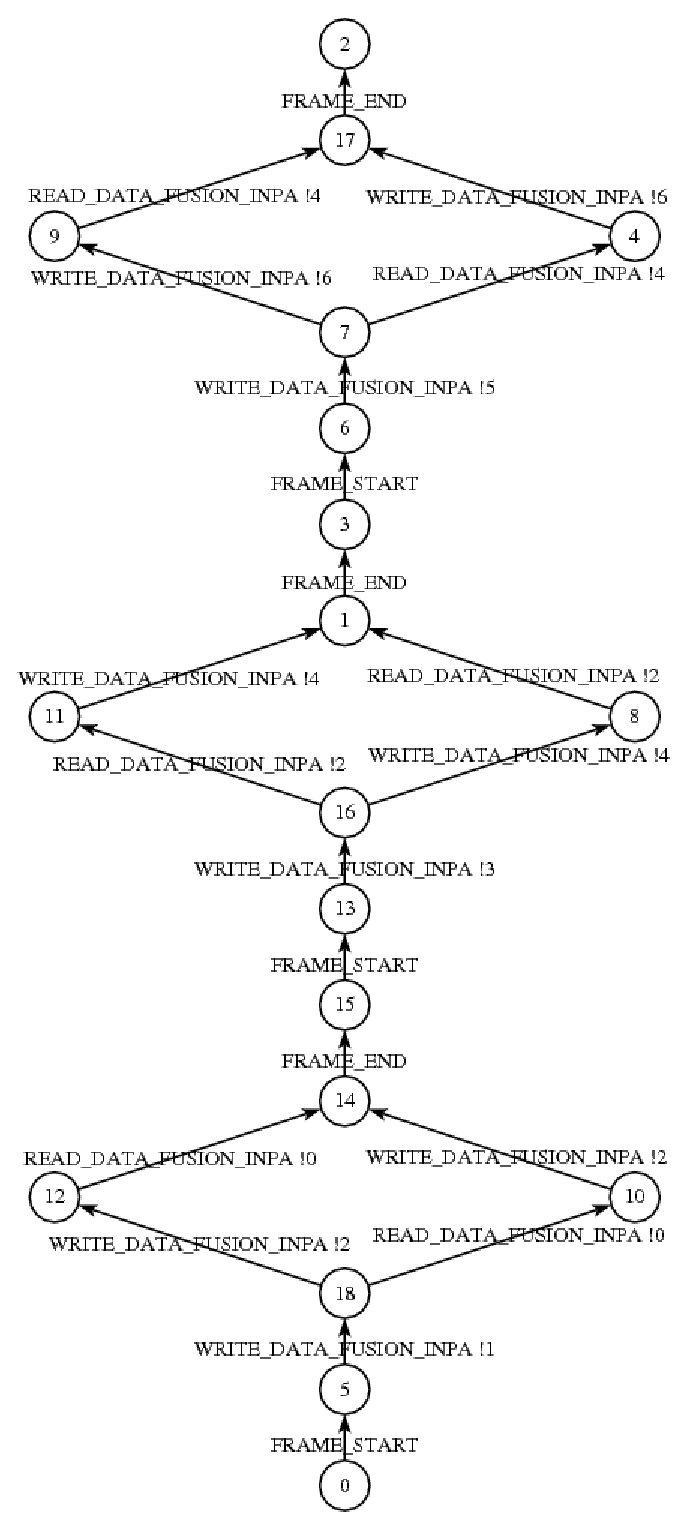
\includegraphics[angle=90, scale=0.4]{../figs/lotos_lts_ex1}$
  \end{center}
}

\subsection{Higher-order DBX}

\frame {
  \frametitle{Higher order sampling}
  \textbf{Higher order DBX}
  \begin{itemize}
    \item Same principle as simple DBX
    \item Instead of double buffer, have a queue
    \item Instead of buffer copy, ``promote'' members of the queue
    \item New AADL property, \texttt{Hyperperiod\_Age}
  \end{itemize}
  \pause
  \begin{center}
    $\includegraphics[scale=0.75]{../figs/ho-exch}$
  \end{center}
}  

\frame {
  \frametitle{Possible use}
  Consider the second-order filter
  \begin{displaymath}
    H(z) = \frac{az^2 + bz + c}{z^2 + dz + e}
  \end{displaymath}
  \pause
  Output can be written as
  \begin{displaymath}
    y = ax + (bx-dy)z^{-1} + (cx-ey)z^{-2}
  \end{displaymath}
  \pause
  Cannot be implemented using regular DBX connector

  Implemented as an AADL design as
  \begin{center}
    $\includegraphics[scale=0.7]{../figs/ho-example}$
  \end{center}
}


\section{Formal semantics}

\subsection{Rationale}

\frame {
  \frametitle{Why formal semantics}
  \begin{itemize}
    \item Allow a mathematical treatment of the system under
      consideration
    \item Allow reasoning based on the mathematical model
    \item We used Structured Operational Semantics (SOS)
    \item SOS describes system evolution as transitions
    \item Each transition has \alert{antecedents} and
      \alert{consequents}
    \item Antecedent describe the preconditions for transition
    \item Consquents describe the transition itself
  \end{itemize}
}

\subsection{Static semantics and Ravenscar Meta-model}

\frame {
  \frametitle{Static semantics}
  \begin{itemize}
    \item Gives the rules for the well-formedness of entities
    \item Uses set theory concepts to describe the entities
    \item The static semantics corresponds to the RMM
  \end{itemize}
  
  \begin{minipage}{0.45\linewidth}
    {\footnotesize
      \begin{eqnarray}
        \nonumber
        \text{\textbf{Periodic tasks}} \ {\cal T}_p \!& \!= \!&\! \{P_1 \ldots P_n\}\\
        \nonumber
        \text{\textbf{Sporadic tasks}} \  {\cal T}_s  \! & \!= \! & \!  \{S_1  \ldots S_m\} \\
        \nonumber
        \text{\textbf{Interrupts}} \   {\cal U} \! & \!= \! & \! \{U_1  \ldots U_k\}  \\ 
        \nonumber
        \text{\textbf{Synchronisers}} \    {\cal D} \! & \!= \! & \! \{D_1 \ldots D_l\} \\  
        \nonumber
        \text{\textbf{Exchangers}} \  {\cal E} \! & \!= \! & \! \{E_1  \ldots E_r\} 
      \end{eqnarray}
    }
  \end{minipage}
  \hspace{2mm}
  \begin{minipage}{0.45\linewidth}
    {\footnotesize
      \begin{eqnarray}
        \nonumber
        \text{\scshape priority}: &{\cal C} & \to \ \ 
             {\scriptstyle \mathbb{ANYPRIORITY}} \\
        \nonumber
        \text{\scshape holdingtime}: & {\cal T} & \to \ \  
             {\scriptstyle \mathbb{TIME}} \\
        \nonumber
        \text{\scshape wcet}: & {\cal A}  &  \to \ \  
             {\scriptstyle \mathbb{TIME}} \\
        \nonumber
        \text{\scshape deadline}: & {\cal A}   &  \to  \ \  
             {\scriptstyle \mathbb{TIME}} \\
        \nonumber
        \text{\scshape prog}: & {\cal C}  & \to \ \  
             {\scriptstyle \mathbb{PROGS}} 
      \end{eqnarray}
    }
  \end{minipage}
}

\frame {
  \frametitle{RMM}
  \begin{center}
    $\includegraphics[scale=0.4]{../figs/rmm}$
  \end{center}
}

\frame {
  \frametitle{Topological definitions}
  {\footnotesize
  \begin{eqnarray}
    \nonumber
    \text{\emph{sets}} & : & \rset \ \subset\  \ {\cal A} \times {\cal
      E} \\
    \nonumber
    \text{\emph{gets}} & : & \rget \ \subset \ \ {\cal T} \times {\cal
      E}  \\
    \nonumber
    \text{\emph{sends\_event}} & : &  \rsvt \  \subset \ \ {\cal A}
    \times {\cal D} \\
    \nonumber
    \text{\emph{awaits\_event}} & : &  \rgvt \ \subset \ \ {\cal T}_s
    \times {\cal D}
  \end{eqnarray}
  }
}

\subsection{Dynamic semantics \& system evolution}

\frame {
  \frametitle{Structured Operational Semantics}
  \begin{itemize}
    \item Labelled transition system
    \item Has preconditions to describe system state that exists
    \item Takes an action, changes system variables (from static
      semantics)
    \item Reaches a new state
  \end{itemize}
  \pause
  \begin{center}
    {\footnotesize
    \formatreg{
      \regle{ \textit{Antecedents}}
	    {
	      \text{\small  \textit{IL}} \intrupt 
	      \big[ 
	        c, R, B, \text{\sffamily ns}, \text{\sffamily t} 
	        \big]
	      \Faitv{\textit{act}}
	      \text{\small  \textit{IL'}} \intrupt
	      \big[ 
	        c', R,' B', \text{\sffamily ns'}, 
	        \text{\sffamily t}
	        \big] \sqplus \delta(\textit{\small act})
	    } \textit{\scriptsize SHORT NAME}
    }
    }
  \end{center}
}

\frame {
  \frametitle{Example transition}
  Models the preemption by the scheduler of a task that is \emph{not}
  the idle task\\

  \formatreg {
    \regle {
      c\neq\iota\ \wedge\ c\neq \sigma\ \wedge\ c\neq
      \sigma_s\ \wedge\ c=a\ \wedge\ \text{\sffamily t}=\text{\sffamily ns} 
    } {
      \big[c, R, B, \text{\sffamily ns}, 
        \text{\sffamily t} 
        \big]
      \Faitv{\text{as}}
      \big[ 
        \sigma, R', B, \text{\sffamily ns}, 
        \text{\sffamily t}
        \big]
      \sqplus 
      \delta(as)\\
      \\
      R' = a\smcirc R
    }
  }
}

\chapter{Conclusions and future work}{``Even if you're on the right
  track,\\you'll get run over if you just sit there.''}{Will Rogers}
\label{chap:conclusions}
Model driven engineering and automatic code generation is a powerful
mechanism for reducing the workload for software development. It is
even more attractive as a methodology when the target domain is
safety-critical and real-time systems. In a nutshell, MDE proposes
that the architecture and design of a system be given in a high-level
language that is then automatically transformed to source code in a
suitable programming language. MDE is particularly attractive for
safety-critical systems for a number of reasons; automatic model to
code transformation ensures the preservation of properties, it reduces
effort which has an impact on the cost, complexity and time needed to
develop a system, and having a high-level model gives the ability to
carry out analyses on the system before it is built.

There are a large number of existing MDE approaches, a few of
which---those specifically targeted to real-time systems---were
presented in Chapter~\ref{chap:biblio}. These include a large class of
formalisms based on UML or an extension thereof, as well as some
proprietary ones such as Lustre/SCADE Suite and Matlab \simu. Each of
these high-level languages provides a certain level of abstraction. 

It was observed that for some, like Simulink and Lustre, the
abstraction level is very high. The design or architecture is very
close to the ``problem space''. In these languages---which seek to
address the problem of developing computer-controlled control
systems---the constructs of the language mirror the methods in which
control algorithms themselves are expressed. The design artifacts are
blocks that perform a transformation on their inputs and provide the
results as outputs. These blocks are connected together via links that
denote the data flows, and which become the inputs upon which the
transformations are carried out and the outputs that result from
them. This is very close to the control loops that are designed using
mathematical functional notations of $y_n = f(x_{n-1}, x_{n-2},
\dots)$. This high level of abstraction, while beneficial for the
specific problem domain within real-time systems, is quite far removed
from the ``solution space''. The solution space in this case being the
runtime entities that actually execute on a physical computer to
approximate the behavior of the system as described in the
model. These runtime entities are the processes and threads, the
message buffers and mutexes, the procedures and their parameters etc.;
in essence, the computing portion of the big picture. Because of this
vertical distance between the architecture and the final source code,
it can be difficult for the designer to realize the implications,
impacts and consequences of design decisions. Also, these approaches
remain quite restrictive as far as the implementation of
general-purpose real-time systems is concerned. It would be a very
tortuous exercise indeed, to build a C$^4$I (Command, Control,
Computers, Communication and Intelligence) system using Simulink or
SCADE Suite.

On the other end of the spectrum are UML based approaches. UML in its
basic vision is for designing software, hence it is tightly coupled
with the object oriented method of software engineering. Its main
entities are classes and relations among those classes. With the newer
versions of UML, there has been a push towards including execution
level artifacts such as threads into the language. This is done by
overloading the basic semantics of the class entity of the
language. This semantic overload leads to considerable confusion and
to counter-intuitive code generation: is an ``active class'' a class
or a thread? Why isn't the code generated for an active class actually
a class? The profiles of UML specifically targeted to the real-time
domain such as HRT-UML and MARTE engage in further semantic overload
by stipulating that stereotypes can specify that a class is not just a
thread, but a periodic thread, or even a shared message buffer, or a
complete executable component.

It was argued in Chapter~\ref{chap:code_gen} that the Architecture
Analysis \& Design Language provides a better level of abstraction. It
is a domain specific language so there is no question of overload. It
allows block structured modeling but uses execution level constructs
at model level such as processes, threads and subprograms. This,
coupled with the ability to use data ports and event (data) ports
provides an attractive level and style of abstraction for real-time
systems.

The Ada programming language, with its strong typing, modularization,
robust runtime with safety features and the inclusion of tasking and
communication primitives at the level of the language makes it an
attractive choice for real-time systems. This, together with the
definition of the Ravenscar Profile for High-integrity Systems---as
outlined in Chapter~\ref{chap:aadlrs}---and its implementation in the
form of the free ORK kernel and the commercial RAVEN kernel from
Aonix, makes for a compelling case for its use in modern systems. In
fact, Pratt \& Whitney have used the RAVEN kernel for the FADEC
(Full-Authority Digital Engine Control) of their new PW6000 jet
engine~\cite{raven-fadec}.

The major thrust of this research work has been the elaboration of
code generation rules from AADL toward Ravenscar-compliant Ada source
code. The main part of this work, as presented in
Chapter~\ref{chap:code_gen}, obviates a lot of the tedious and
error-prone work of coding a framework in Ada that provides the
non-functional substrate for solving the functional part of the
real-time problem at hand. The automatic code generation saves time
and difficult-to-identify errors in the construction of the
framework. The AADL itself is eminently suited to this kind of
development by providing---as stated---direct representations for
processes, threads and subprograms; and also some indirect
abstractions such as ports and connections between threads. This
brings the best of both worlds together and allows architecture
modeling where the designer can see the consequences of his decisions
on the execution entities generated as well as providing abstractions
for conceptual design of applications.

A major issue in writing control systems that have different
functionalities running at different periods is that all communication
between various jobs must be deterministic. While this is easy to
achieve in a synchronous system running on a cyclic executive---case
in point being Lustre/SCADE Suite and Simulink---it can be tricky in
case a full process-based executive is
used. Chapter~\ref{chap:adv_code} presented a mechanism to produce
deterministic communication constructs automatically from an AADL
description. This, coupled with the automatic verification code
generated in LOTOS, is a step in the direction for creating AADL and
Ada Ravenscar based certifiable control systems.

A formal semantics for the generated Ada code running on a
Ravenscar-compliant executive was given in
Chapter~\ref{chap:formal_sem}. The static semantics were given in set
theoretic notation and the dynamic semantics in the form of Structural
Operational Semantics rules, which manipulate and modify the system
data structures depending on the transitions taken to model the
system's evolution over time.

\section{Self-criticism}
In any scientific endeavor, it is easy---and dangerous---to overlook
or ignore the potential disadvantages of what is being
proposed. Therefore, in this section a few criticisms are leveled at
the work that has been presented. The most important facility yet
lacking in the presented approach is that of distribution. There is no
restriction in the Ravenscar computation model that would preclude the
possibility of having different tasks executing on different physical
processors connected via a communication medium. There is also the
possibility of having a partitioned Ravenscar system in the manner of
the ARINC 653 specification~\cite{arinc}. In fact, some work towards
this end has already been done~\cite{tokar@adalett03} using such
partitioned systems with Ada application-level programs.

Distributed Ravenscar application development is already being
explored via the development of a lightweight distribution middleware
called PolyORB~\cite{zalila@ae07}. This middleware, which is
completely Ravenscar-compliant, can be used to write distributed, hard
real-time systems that conform to the Ravenscar Profile's
computational model. Distributed communication is only done via
message passing, never with synchronous RPC in order to preserve the
semantics of the profile.

Another area that is lacking is that of the capability to specify
``real-time transactions''~\cite{cornwell@ae96}. A real-time
transaction is a conceptual notion of the response of a system to an
event, whether that response is completely provided by one thread
within the system, or by a number of cooperating and communicating
threads. In case the response to an event is to be computed by a
number of threads, the transaction is considered to be the entire
control and data flow between the reception of the event, and action
taken by the system till the event is treated and an output at the
final thread is available. Modeling of transactions is important
because it allows the calculation of a response time that is more
systemic than that of a single thread, since now the entire path of
the treatment of the event through the system can be analyzed,
including the attendant computation times, up until the end of
treatment. This notion is especially useful in the case of control
systems, where the ``event'' would be the dispatching of the periodic
thread that starts the control loop's function by reading sensors, and
the final thread is the one(s) that write(s) commands to the
actuator(s).

There are certain restrictions that are inherent to the Ravenscar
Profile itself, such as the absence of RPC communication between
threads, the inability to signal multiple threads simultaneously (this
is a consequence of having at most one entry per protected object and
at most one task waiting on that entry), and no dynamic creation or
destruction of tasks. These restrictions, however, are more of an
advantage than a disadvantage as they ensure safe and robust operation
of the system.

The verification mechanism implemented, as described in
Chapter~\ref{chap:adv_code} could be improved. At the moment, the
scheduler is not explicitly modeled in the LOTOS code generated,
instead, its functionality is subsumed by the LOTOS processes that
model the threads. A cleaner and more easy to understand approach
would be to generate a separate LOTOS process for the scheduler that
sends events to the various threads at the correct points to enable
them for execution.

The formal semantics as described in Chapter~\ref{chap:formal_sem}
have not been implemented in a suitable language such as AsmL, or
indeed any other convenient formalism. For the provided semantics to
be of engineering use---rather than a documentation aid or a purely
academic exercise---they need to be implemented. The uses and
advantages to having an implemented semantics are myriad, and have
already been discussed.

A minor point is that the transformation rules from AADL to RMM within
the ARC code generator have been written in Java. Although this is a
valid method of implementation, currently there are specialized model
transformation languages available that greatly ease the specification
and implementation of such transformations. One such language, which
is implemented for the EMF framework provided with Eclipse, is the
Atlas Transformation Language (ATL)~\cite{jouault@oopsla06}. It was
not used since at the time ARC was started, ATL was still in its alpha
phase and was not very usable.

\section{Future work}
There are a few axes of research and engineering activity that are a
logical sequel to the work under discussion. Among these activities,
some are purely engineering endeavours, others are purely research,
and some activities have an overlap. In this section a few of these
open questions are addressed and possible future avenues of work are
enumerated.

It is patently obvious that the issues mentioned in the previous
section as criticisms of the work presented are open to
improvement. Of these, code generation for distributed Ravenscar
systems and an ARINC 653 compliant real-time operating system together
with code generation tooling is already being pursued within the
author's own research group.

A major axis of exploration will be opened up via the implementation
of the formal semantics of generated Ravenscar systems as
described. This semantics, once implemented in a formal description
language, could potentially be used for verification via model
checking as well as simulation to aid in the analysis of systems while
still at the design stage.

A separate plugin is also envisaged that can provide code reporting and
documentation information for the generated code. The code generation
rules as presented allow for the direct identification of the source
artifact(s) to which a piece of code corresponds, and vice-versa. A
hypertext report generator that can provide a concise traceability
graph between the architecture model artifacts and their resulting
code can be very useful for certification purposes, specially in the
context of the aerospace industry since the DO-178B standard does
stipulate strict traceability requirements.

A major research avenue is the study of whether and how a synchronous
paradigm such as Lustre could be used in conjunction with AADL. It is
possible to envisage that the response code for each thread be written
not in Ada or C, but in the form of a Lustre node. Each time the
thread is dispatched, it would in fact run the main Lustre node that
corresponds to its response code. The input flows to the main node
would be the \texttt{in data port} features and the output flows would
be the \texttt{out data port} features as defined by the thread. This
could lead to a fusion of the architecture description language
approach with the synchronous approach.

The---approximately---inverse of the previous proposal can also be
considered. Compiling a functional model such as that provided by
Simulink towards the Ada programming language to run on top of a
Ravenscar-compliant RTOS can be useful. Collapsing Simulink blocks at
the same ``rate'' into one Ada task of the same period with Simulink
data connections being represented by AADL data ports is feasible. The
thread callbacks in this case would be automatically generated via an
analysis of the blocks that have been collapsed into it.

%%% Local Variables:
%%% mode: latex
%%% mode: flyspell
%%% TeX-master: t
%%% End:


\end{document}
